\chapter{Tutorial 4: Meshing}

To get a volume mesh from tomographic data you first have to define how many elements your surface mesh should have.
To create the volume mesh you need the precalculated surface mesh and the radius-edge ratio.
After the creation it's important to measure the quality of the generated mesh. 
There are different types of quality mesh measures. 
For more details look on the TetGen homepage (http://wias-berlin.de/software/tetgen/features.html).

In this tutorial the measures "edgeRatio", "volume" and "minAngle" are used.
A python script example can be found in "/examples/MeshExample/Liver/liverMesh\_runner.py". 
This script first creates a surface mesh with 1800 point cells. 
After that a volume mesh is generated with a radius-edge ratio of 1.4.
This mesh is then used for testing the measures mentioned above.
In order to run this example from the command line please first make sure that the MSML source is in your Python path:
\begin{lstlisting}[language=sh, breaklines=true]
$ export PYTHONPATH="$PYTHONPATH:/opt/msml/src"
\end{lstlisting}

Then change to the folder that contains the script

\begin{lstlisting}[language=sh, breaklines=true]
$ cd /opt/msml/examples/MeshExample/Liver
\end{lstlisting}

and run it:

\begin{lstlisting}[language=sh, breaklines=true]
$ python liverMesh_runner.py
\end{lstlisting}

Use ParaView to view the result and inspect the mesh. 
You can start ParaView with the following:
\begin{lstlisting}[language=sh, breaklines=true]
$ cd /opt/paraview/bin
\end{lstlisting}
\begin{lstlisting}[language=sh, breaklines=true]
$ ./paraview
\end{lstlisting}

Now create volume meshes with an radius-edge ratio of 5 and 20.
For this you have to change the parameter \emph{maxEdgeRadiusRatio} in the given script.
Also view the results in ParaView and take a screenshot for every mesh.
How do the meshes differ? 
Compare the quality mesh measures from the python script as well.

Also try the filter function \emph{Extract Cells By Region} as shown in Fig. \ref{ParaviewFilterScreenshot}. 
Don't forget to push the \emph{Apply} - button. 
Take also a screenshot for each filtered mesh.

\begin{figure}[h]
  	\centering
    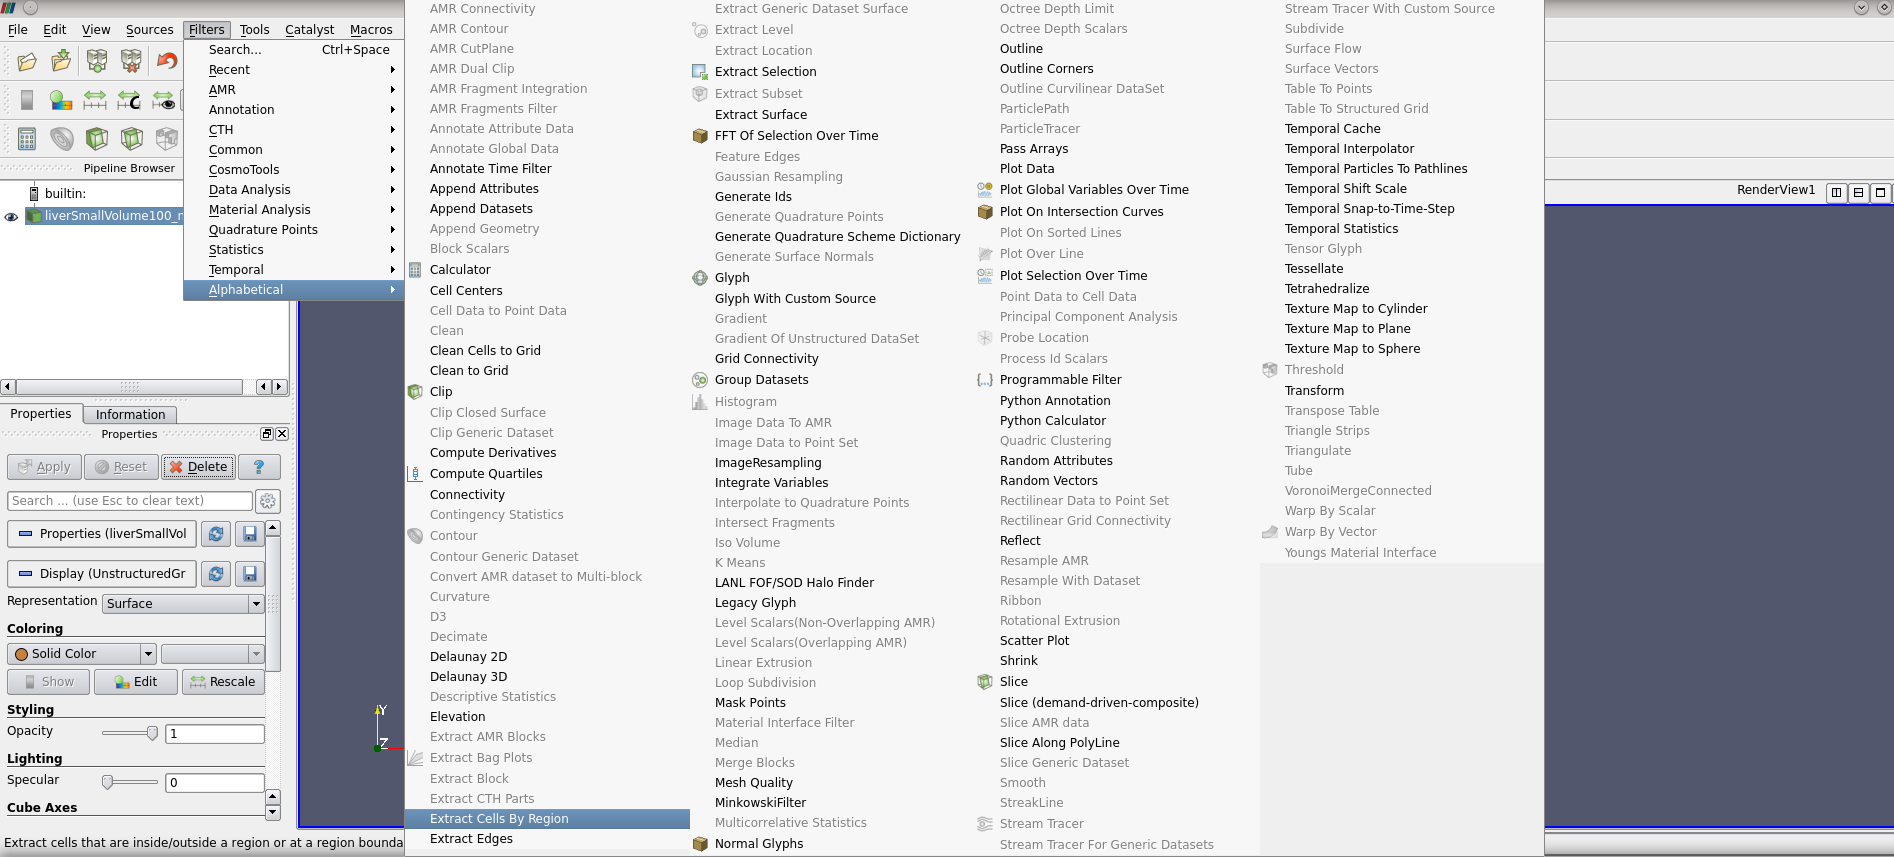
\includegraphics[width=\textwidth]{pictures/paraview_filter.png}
    \caption{Get filter preferences in ParaView.}
    \label{ParaviewFilterScreenshot}
\end{figure}

Now create a volume mesh with 100 point cells.
How do the generated mesh and the mesh with 1800 point cells differ (optically, quality mesh measures)?